\documentclass{standalone}
\usepackage{tikz}
\usepackage{tikz-cd}
\usepackage{tikz-3dplot}
\usepackage{pgfplots}
\usepackage{pgffor} % For \foreach loop
\pgfplotsset{compat=newest} % Adjust to your version of pgfplots
\def\Circlearrowleft{\ensuremath{%
		\rotatebox[origin=c]{180}{$\circlearrowleft$}}}
\def\Circlearrowright{\ensuremath{%
		\rotatebox[origin=c]{180}{$\circlearrowright$}}}
\def\CircleArrowleft{\ensuremath{%
		\reflectbox{\rotatebox[origin=c]{180}{$\circlearrowleft$}}}}
\def\CircleArrowright{\ensuremath{%
		\reflectbox{\rotatebox[origin=c]{180}{$\circlearrowright$}}}}
\usetikzlibrary{
	3d, % For 3D drawing
	angles,
	arrows,
	arrows.meta,
	backgrounds,
	bending,
	calc,
	decorations.pathmorphing,
	decorations.pathreplacing,
	decorations.markings,
	fit,
	matrix,
	patterns,
	patterns.meta,
	positioning,
	quotes,
	shadows,
	shapes,
	shapes.geometric
}

\begin{document}
	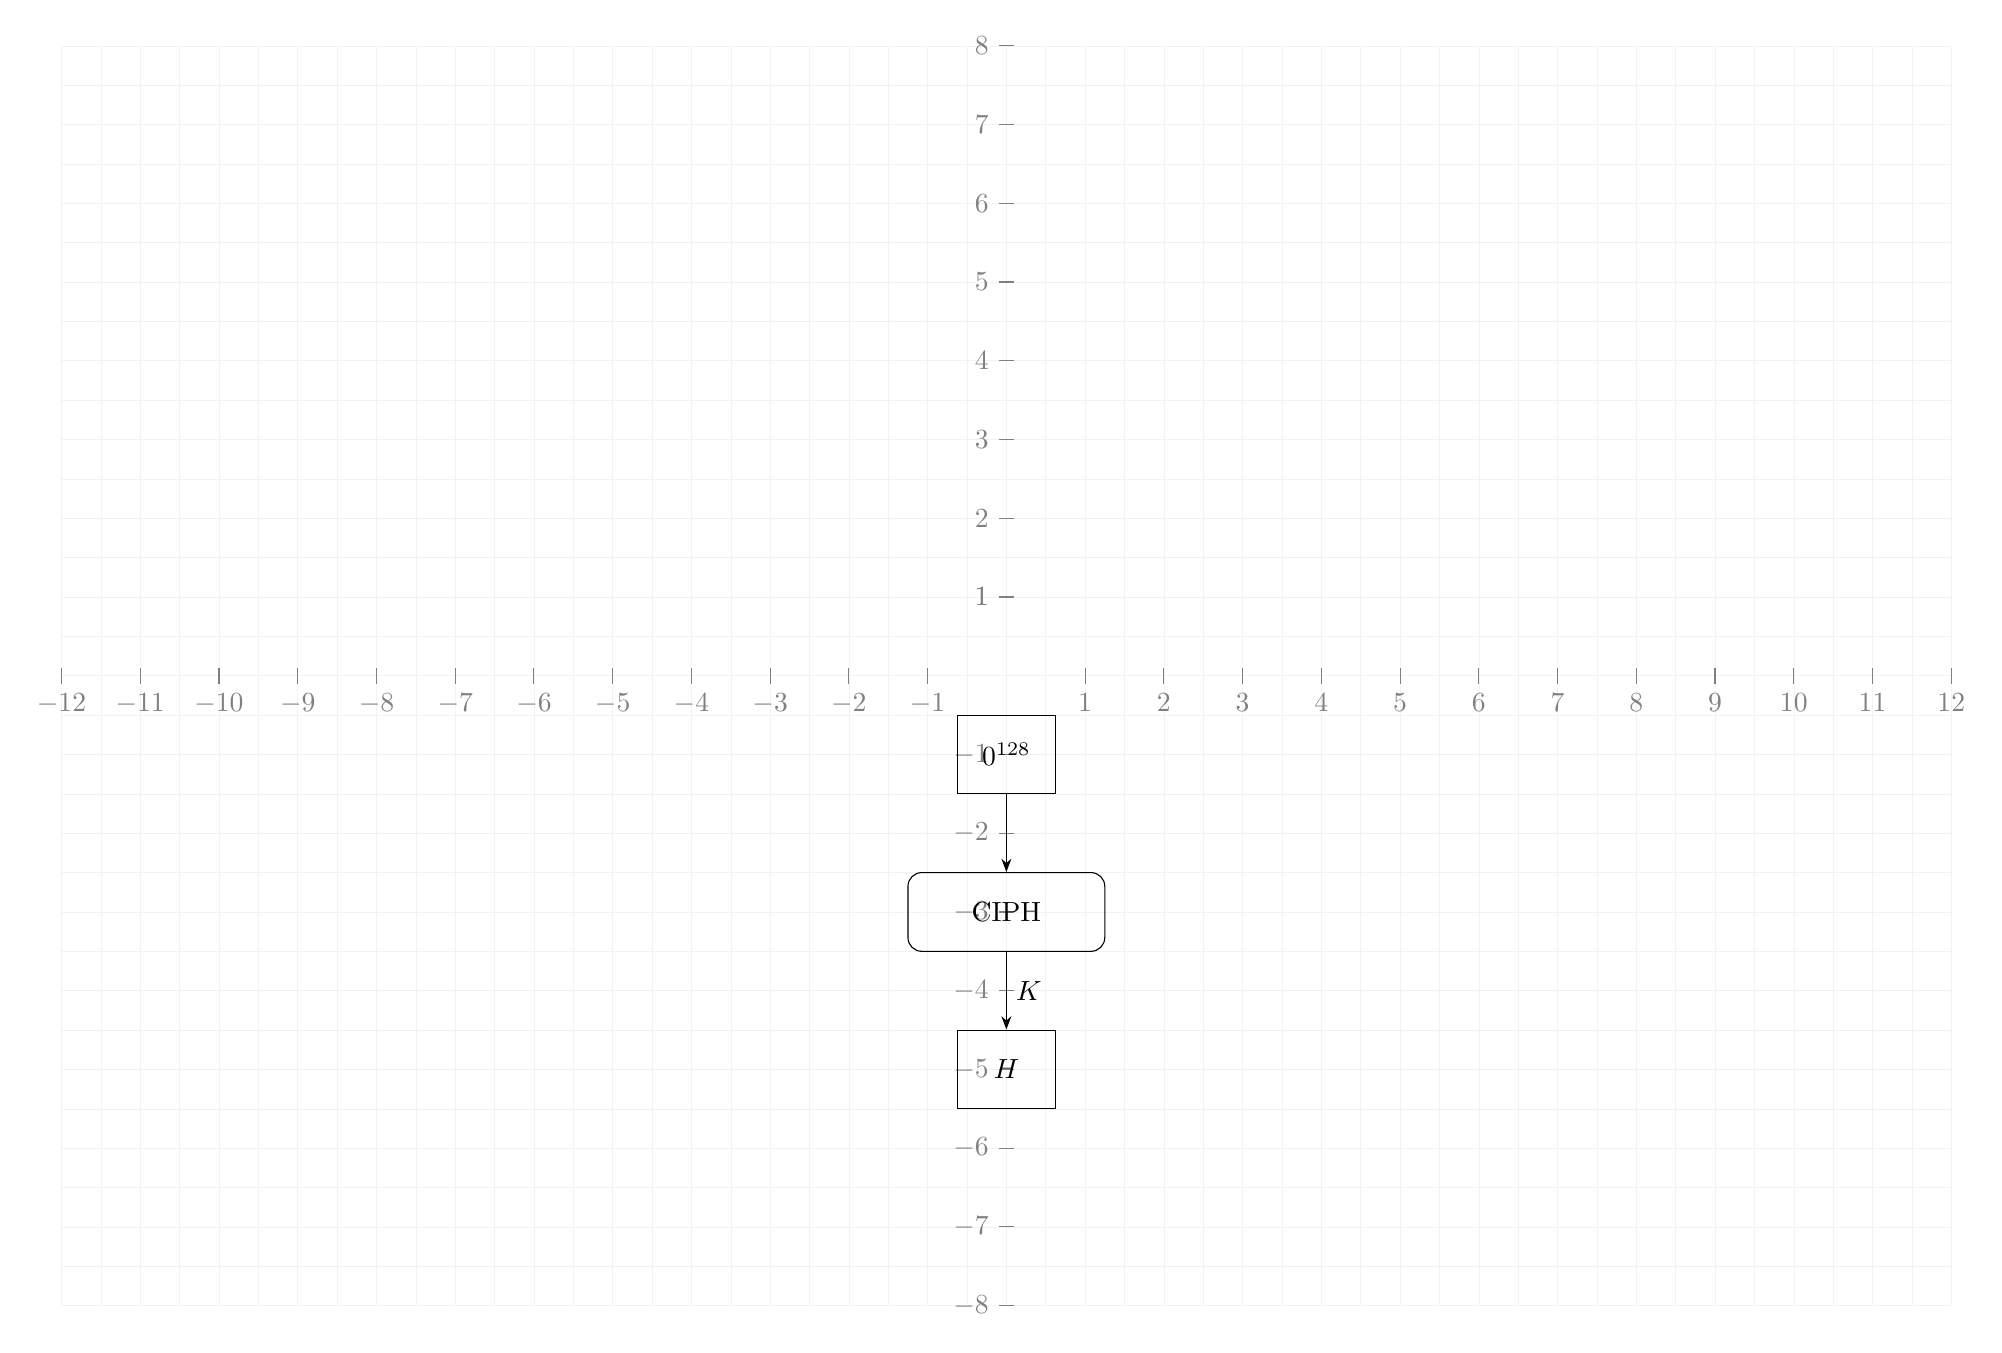
\begin{tikzpicture}[>=Stealth]
		\def \x{12}
		\def \y{8}
		\draw[very thin,color=gray!10,step=.5] (-\x,-\y) grid (\x,\y);
		
		\foreach \i in {-\x,...,-2,-1,1,2,...,\x}
		\draw[gray] (\i,.1)--(\i,-.1) node[below] {$\i$};%x-axis
		\foreach \i in {-\y,...,-2,-1,1,1,2,...,\y}
		\draw[gray] (.1,\i)--(-.1,\i) node[left] {$\i$};%y-axis
		
		
		\node[draw, rectangle, minimum width=1.25cm, minimum height=1cm] (zero) at (0,-1) {$0^{128}$};
		\node[draw, rectangle, rounded corners=5pt, minimum width=2.5cm, minimum height=1cm] (ciph) at (0,-3) {$\textnormal{CIPH}$};
		\node[draw, rectangle, minimum width=1.25cm, minimum height=1cm] (H) at (0,-5) {$H$};
		
		% Arrows
		\draw[->] (zero) -- (ciph);
		\draw[->] (ciph) -- (H) node[midway, right] {$K$};
		
	\end{tikzpicture}
\end{document}